\exercisesheader{}

% 17 - regression_units

\eoce{\qt{Units of regression\label{regression_units}} Consider a regression 
predicting weight (kg) from height (cm) for a sample of adult males. 
What are the units of the correlation coefficient, the intercept, 
and the slope?
}{}

% 18 - which_higher_scatter

\eoce{\qtq{Which is higher\label{which_higher_scatter}} Determine if I or II 
is higher or if they are equal. Explain your reasoning.
\noindent For a regression line, the uncertainty associated with the 
slope estimate, $b_1$, is higher when
\begin{enumerate}
\item[I.] there is a lot of scatter around the regression line or
\item[II.] there is very little scatter around the regression line
\end{enumerate}
}{}

% 19 - residual_apple_weight

\eoce{\qt{Over-under, Part I\label{residual_apple_weight}} Suppose we fit a 
regression line to predict the shelf life of an apple based on its weight. 
For a particular apple, we predict the shelf life to be 4.6 days. The 
apple's residual is -0.6 days. Did we over or under estimate the 
shelf-life of the apple? Explain your reasoning.
}{}

% 20 - residual_sun_cancer

\eoce{\qt{Over-under, Part II\label{residual_sun_cancer}} Suppose we fit a 
regression line to predict the number of incidents of skin cancer per 
1,000 people from the number of sunny days in a year. For a particular 
year, we predict the incidence of skin cancer to be 1.5 per 1,000 people, 
and the residual for this year is 0.5. Did we over or under estimate 
the incidence of skin cancer? Explain your reasoning.
}{}

% 21 - tourism_spending_reg_conds

\eoce{\qt{Tourism spending\label{tourism_spending_reg_conds}} The Association of 
Turkish Travel Agencies reports the number of foreign tourists 
visiting Turkey and tourist spending by year.
\footfullcite{data:turkeyTourism} Three plots are provided: 
scatterplot showing the relationship between these two variables 
along with the least squares fit, residuals plot, and histogram of 
residuals.
\begin{center}
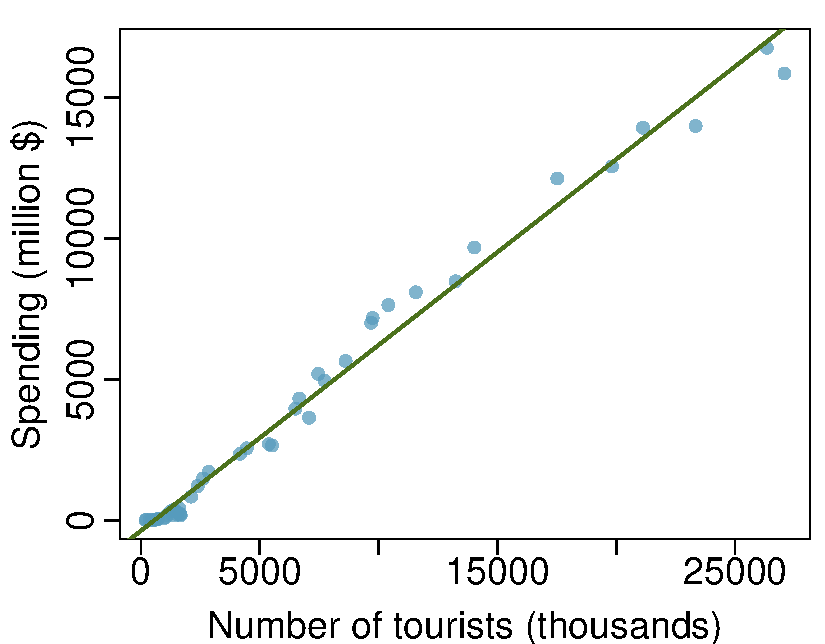
\includegraphics[width=0.32\textwidth]{ch_regr_simple_linear/figures/eoce/tourism_spending_reg_conds/tourism_spending_count.pdf}
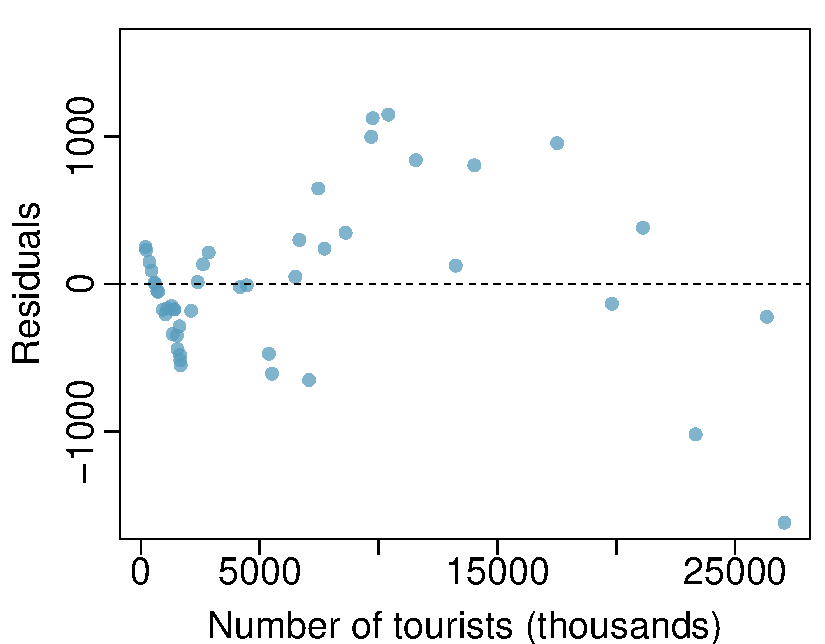
\includegraphics[width=0.32\textwidth]{ch_regr_simple_linear/figures/eoce/tourism_spending_reg_conds/tourism_spending_count_residuals.pdf}
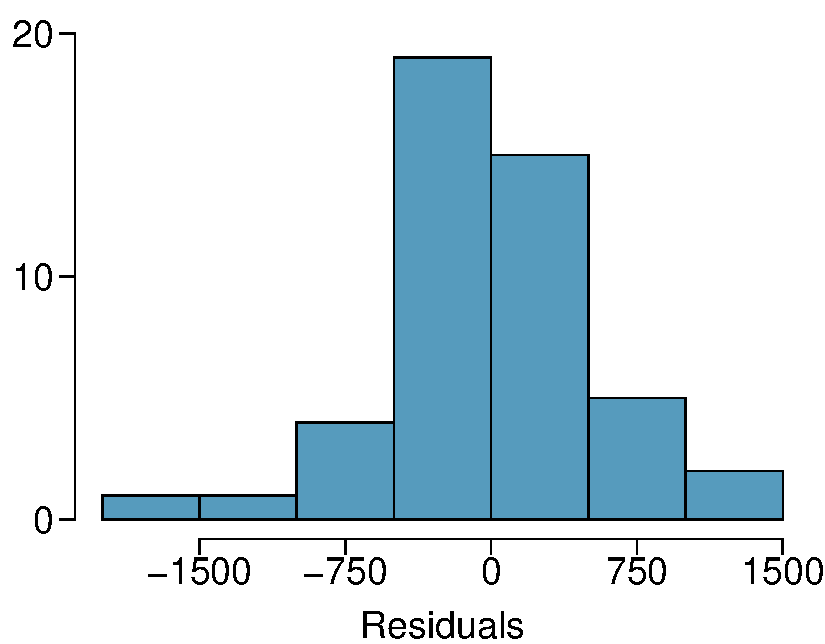
\includegraphics[width=0.32\textwidth]{ch_regr_simple_linear/figures/eoce/tourism_spending_reg_conds/tourism_spending_count_residuals_hist.pdf}
\end{center}
\begin{parts}
\item Describe the relationship between number of tourists and spending.
\item What are the explanatory and response variables?
\item Why might we want to fit a regression line to these data?
\item Do the data meet the conditions required for fitting a least squares 
line? In addition to the scatterplot, use the residual plot and histogram 
to answer this question. 
\end{parts}
}{}

% 22 - starbucks_cals_carbos

\eoce{\qt{Nutrition at Starbucks, Part I\label{starbucks_cals_carbos}} 
The scatterplot below shows the relationship between the number of 
calories and amount of carbohydrates (in grams) Starbucks food menu 
items contain.\footfullcite{data:starbucksCals} Since Starbucks only 
lists the number of calories on the display items, we are interested 
in predicting the amount of carbs a menu item has based on its 
calorie content.
\begin{center}
\tabspecial{tableau-starbucks-p1}{
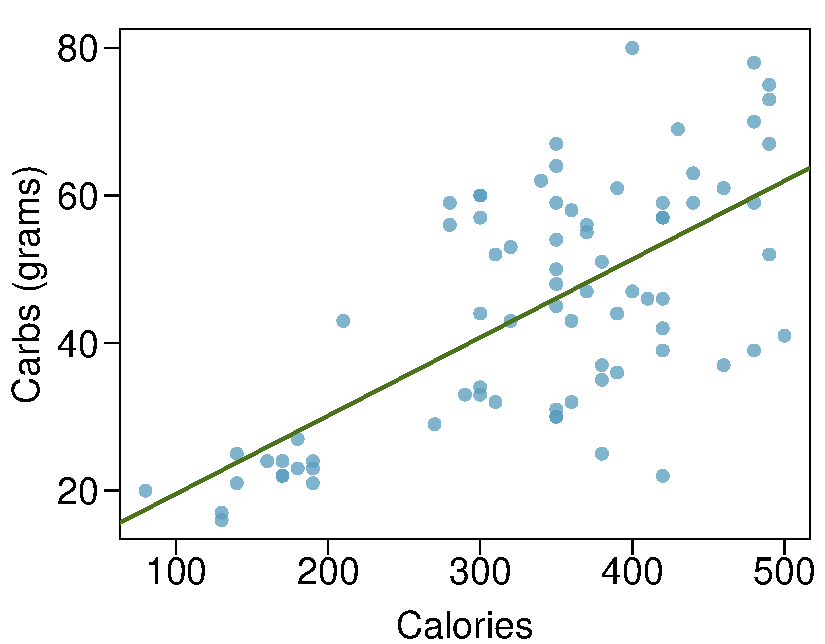
\includegraphics[width=0.32\textwidth]{ch_regr_simple_linear/figures/eoce/starbucks_cals_carbos/starbucks_cals_carbos.pdf}
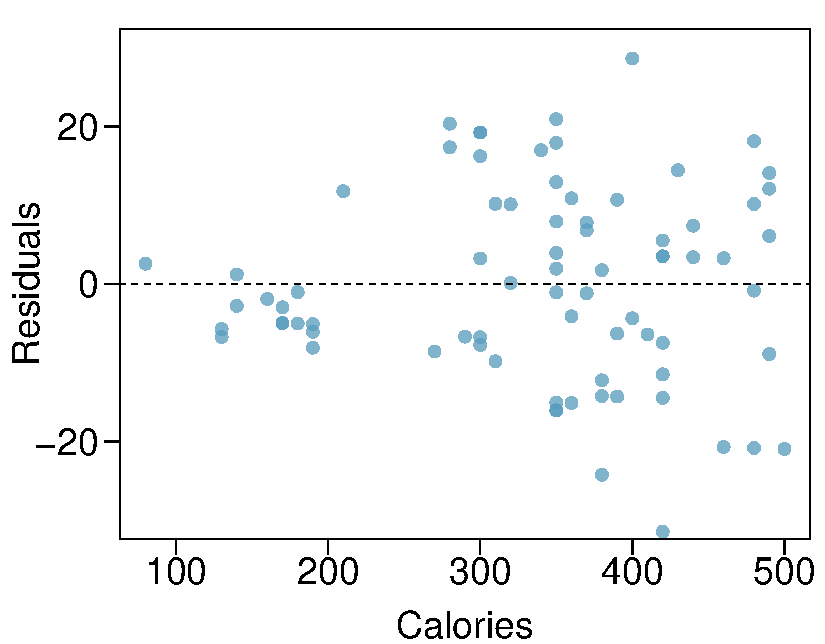
\includegraphics[width=0.32\textwidth]{ch_regr_simple_linear/figures/eoce/starbucks_cals_carbos/starbucks_cals_carbos_residuals.pdf}
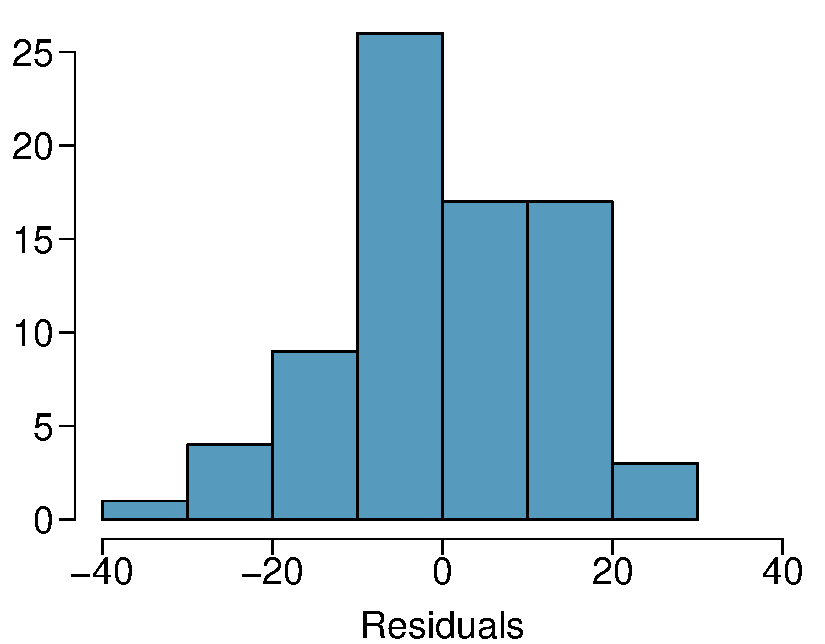
\includegraphics[width=0.32\textwidth]{ch_regr_simple_linear/figures/eoce/starbucks_cals_carbos/starbucks_cals_carbos_residuals_hist.pdf}}
\end{center}
\begin{parts}
\item Describe the relationship between number of calories and amount 
of carbohydrates (in grams) that Starbucks food menu items contain.
\item In this scenario, what are the explanatory and response 
variables?
\item Why might we want to fit a regression line to these data?
\item Do these data meet the conditions required for fitting a least 
squares line?
\end{parts}
}{}

% 23 - coast_starlight_reg

\eoce{\qt{The Coast Starlight, Part II\label{coast_starlight_reg}} \videosolution{ahss_eoce_sol-coast_starlight_reg} 
Exercise~\ref{coast_starlight_corr_units} introduces data on the Coast Starlight 
Amtrak train that runs from Seattle to Los Angeles. The mean travel 
time from one stop to the next on the Coast Starlight is 129 mins, 
with a standard deviation of 113 minutes. The mean distance traveled 
from one stop to the next is 108 miles with a standard deviation of 
99 miles. The correlation between travel time and distance is 0.636.
\begin{parts}
\item Write the equation of the regression line for predicting travel 
time.
\item Interpret the slope and the intercept in this context.
\item Calculate $R^2$ of the regression line for predicting travel 
time from distance traveled for the Coast Starlight, and interpret 
$R^2$ in the context of the application.
\item The distance between Santa Barbara and Los Angeles is 103 
miles. Use the model to estimate the time it takes for the Starlight 
to travel between these two cities.
\item It actually takes the Coast Starlight about 168 mins to travel 
from Santa Barbara to Los Angeles. Calculate the residual and explain 
the meaning of this residual value.
\item Suppose Amtrak is considering adding a stop to the Coast 
Starlight 500 miles away from Los Angeles. Would it be appropriate to 
use this linear model to predict the travel time from Los Angeles to 
this point? 
\end{parts}
}{}

% 24 - body_measurements_shoulder_height_reg

\eoce{\qt{Body measurements, Part III\label{body_measurements_shoulder_height_reg}}
Exercise~\ref{body_measurements_shoulder_height_corr_units} introduces 
data on shoulder girth and height of a group of individuals. The 
mean shoulder girth is 107.20 cm with a standard deviation of 
10.37 cm. The mean height is 171.14 cm with a standard deviation 
of 9.41 cm. The correlation between height and shoulder girth is 0.67.
\begin{parts}
\item Write the equation of the regression line for predicting height.
\item Interpret the slope and the intercept in this context.
\item Calculate $R^2$ of the regression line for predicting height 
from shoulder girth, and interpret it in the context of the 
application.
\item A randomly selected student from your class has a shoulder 
girth of 100 cm. Predict the height of this student using the model.
\item The student from part~(d) is 160 cm tall. Calculate the 
residual, and explain what this residual means.
\item A one year old has a shoulder girth of 56 cm. Would it be 
appropriate to use this linear model to predict the height of this 
child?
\end{parts}
}{}

% 25 - murders_poverty_reg

\eoce{\qt{Murders and poverty, Part I\label{murders_poverty_reg}} \videosolution{ahss_eoce_sol-murders_poverty_reg} The following 
regression output is for predicting annual murders per million from 
percentage living in poverty in a random sample of 20 metropolitan 
areas.\\[2mm]
\begin{minipage}[c]{0.56\textwidth}
{\footnotesize
\begin{tabular}{rrrrr}
    \hline
            & Estimate  & Std. Error    & t value   & Pr($>$$|$t$|$) \\ 
    \hline
(Intercept) & -29.901   & 7.789         & -3.839    & 0.001 \\ 
poverty\%   & 2.559     & 0.390         & 6.562     & 0.000 \\ 
   \hline
\end{tabular}
$s = 5.512 \hfill R^2 = 70.52\% \hfill R^2_{adj} = 68.89\%$ 
}
\begin{parts}
\item Write out the linear model.
\item Interpret the intercept.
\item Interpret the slope.
\item Interpret $R^2$.
\item Calculate the correlation coefficient.
\end{parts}
\end{minipage}
\begin{minipage}[c]{0.02\textwidth}
$\:$\\
\end{minipage}
\begin{minipage}[c]{0.39\textwidth}
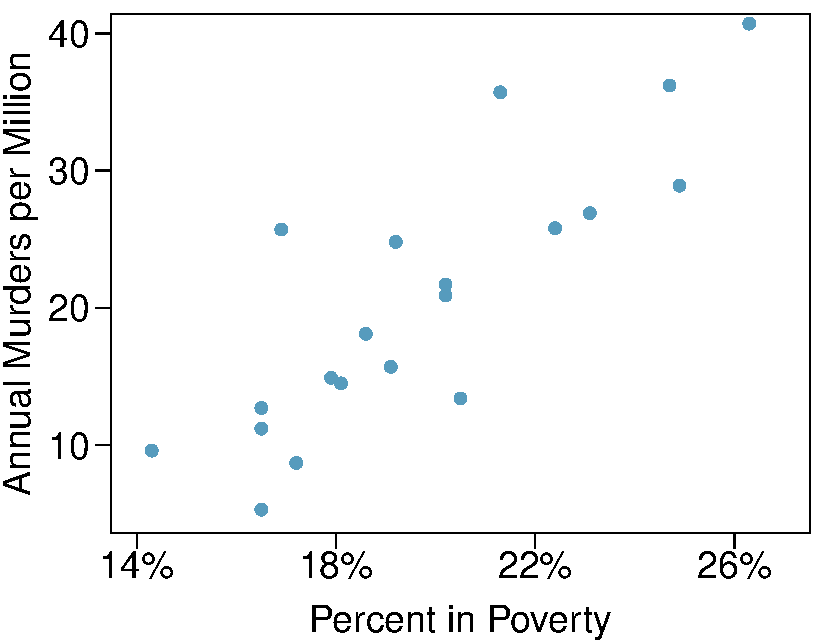
\includegraphics[width=\textwidth]{ch_regr_simple_linear/figures/eoce/murders_poverty_reg/murders_poverty.pdf}
\end{minipage}
}{}

% 26 - cat_body_heart_reg

\eoce{\qt{Cats, Part I\label{cat_body_heart_reg}} The following regression output is 
for predicting the heart weight (in g) of cats from their body weight 
(in kg). The coefficients are estimated using a dataset of 144 
domestic cats.\\[2mm]
\begin{minipage}[c]{0.56\textwidth}
{\footnotesize
\begin{tabular}{rrrrr}
    \hline
            & Estimate  & Std. Error    & t value   & Pr($>$$|$t$|$) \\ 
    \hline
(Intercept) & -0.357    & 0.692         & -0.515    & 0.607 \\ 
body wt     & 4.034     & 0.250         & 16.119    & 0.000 \\ 
    \hline
\end{tabular}
$s = 1.452 \hfill R^2 = 64.66\% \hfill R^2_{adj} = 64.41\%$ 
}
\begin{parts}
\item Write out the linear model.
\item Interpret the intercept.
\item Interpret the slope.
\item Interpret $R^2$.
\item Calculate the correlation coefficient.
\end{parts}
\end{minipage}
\begin{minipage}[c]{0.02\textwidth}
$\:$\\
\end{minipage}
\begin{minipage}[c]{0.39\textwidth}
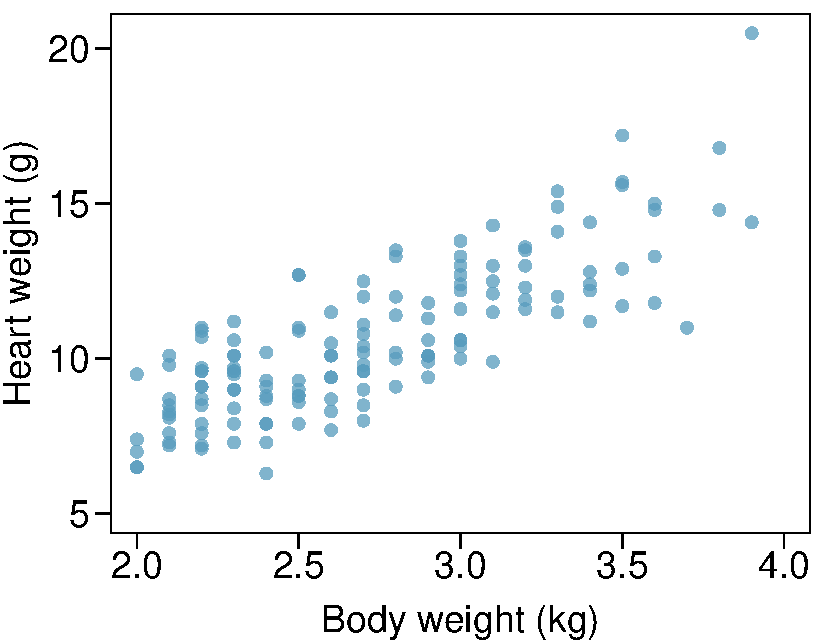
\includegraphics[width=\textwidth]{ch_regr_simple_linear/figures/eoce/cat_body_heart_reg/cat_body_heart.pdf}
\end{minipage}
}{}

% 27 - outliers_1

\eoce{\qt{Outliers, Part I\label{outliers_1}} Identify the outliers in the 
scatterplots shown below, and determine what type of outliers they are. 
Explain your reasoning.
\begin{center}
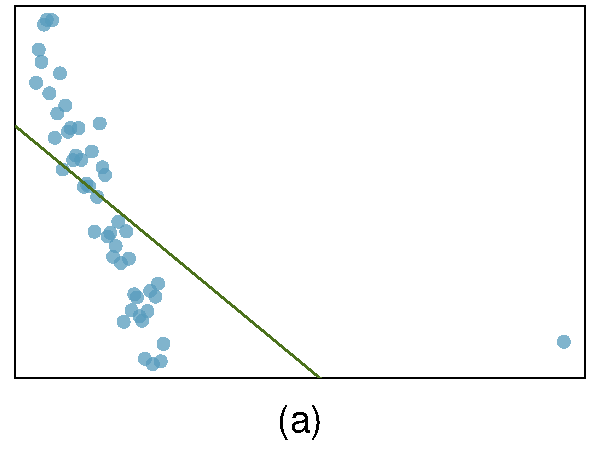
\includegraphics[width=0.32\textwidth]{ch_regr_simple_linear/figures/eoce/outliers_1/outliers_1_influential.pdf}
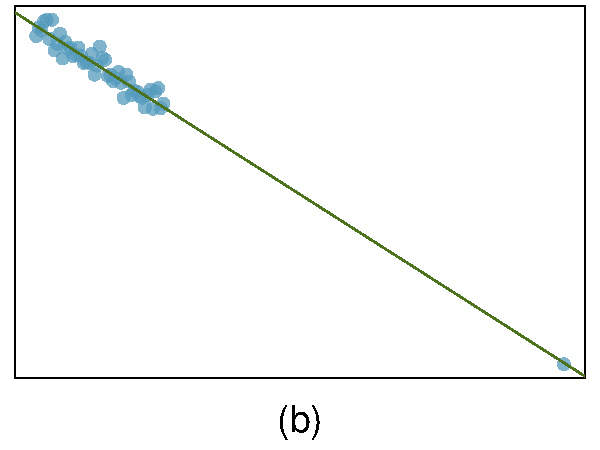
\includegraphics[width=0.32\textwidth]{ch_regr_simple_linear/figures/eoce/outliers_1/outliers_2_leverage.pdf}
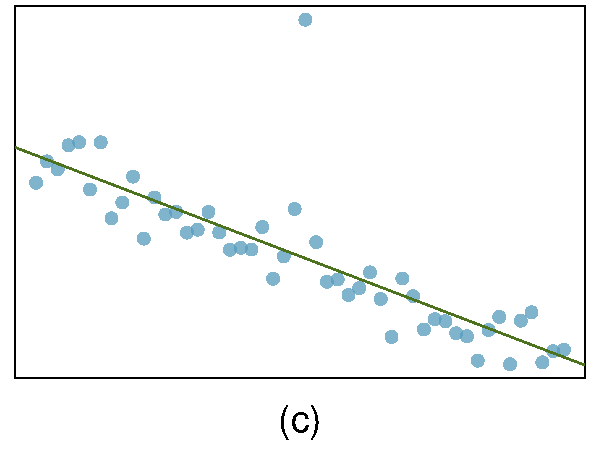
\includegraphics[width=0.32\textwidth]{ch_regr_simple_linear/figures/eoce/outliers_1/outliers_3_outlier.pdf}
\end{center}
}{}

% 28 - outliers_2

\eoce{\qt{Outliers, Part II\label{outliers_2}} Identify the outliers in the scatterplots 
shown below and determine what type of outliers they are. Explain 
your reasoning.
\begin{center}
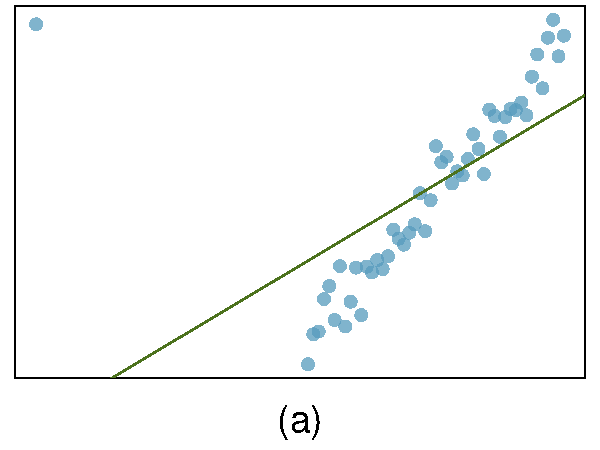
\includegraphics[width=0.32\textwidth]{ch_regr_simple_linear/figures/eoce/outliers_2/outliers_1_influential.pdf}
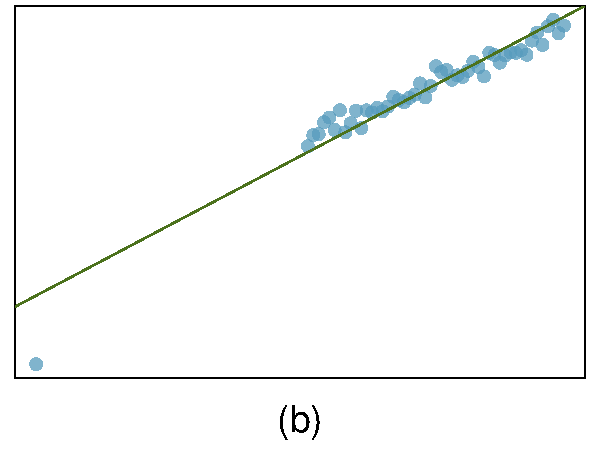
\includegraphics[width=0.32\textwidth]{ch_regr_simple_linear/figures/eoce/outliers_2/outliers_2_influential.pdf}
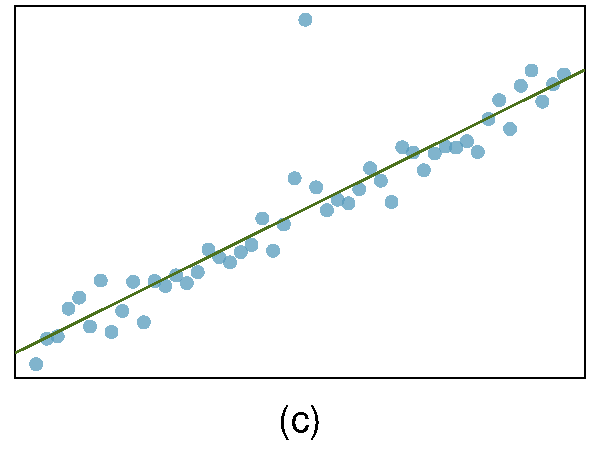
\includegraphics[width=0.32\textwidth]{ch_regr_simple_linear/figures/eoce/outliers_2/outliers_3_outlier.pdf}
\end{center}
}{}

% 29 - urban_homeowners_outlier

\eoce{\qt{Urban homeowners, Part I\label{urban_homeowners_outlier}} The 
scatterplot below shows the percent of families who own their 
home vs. the percent of the population living in urban areas.
\footfullcite{data:urbanOwner} There are 52 observations, each 
corresponding to a state in the US. Puerto Rico and District of 
Columbia are also included.

\noindent\begin{minipage}[c]{0.5\textwidth}
\begin{parts}
\item Describe the relationship between the percent of families who 
own their home and the percent of the population living in urban areas.
\item The outlier at the bottom right corner is District of Columbia, 
where 100\% of the population is considered urban. What type of an outlier 
is this observation?
\end{parts}
\end{minipage}
\begin{minipage}[c]{0.05\textwidth}
$\:$\\
\end{minipage}
\begin{minipage}[c]{0.4\textwidth}
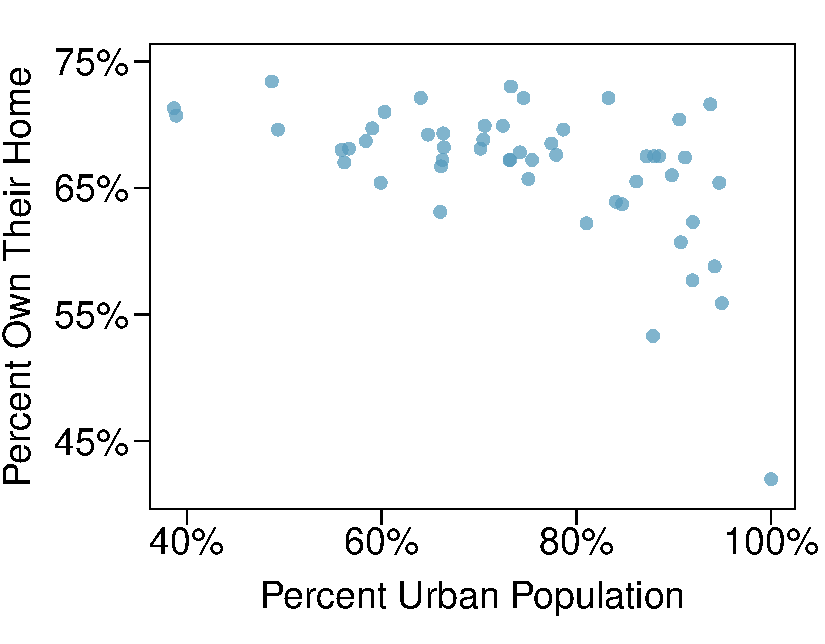
\includegraphics[width=0.95\textwidth]{ch_regr_simple_linear/figures/eoce/urban_homeowners_outlier/urban_homeowners_outlier.pdf} \vspace{-3mm}
\end{minipage}
}{}

% 30 - crawling_babies_outlier

\eoce{\qt{Crawling babies, Part II\label{crawling_babies_outlier}} 
Exercise~\ref{crawling_babies_corr_units} introduces 
data on the average monthly temperature during the month babies first 
try to crawl (about 6 months after birth) and the average first 
crawling age for babies born in a given month. A scatterplot of these 
two variables reveals a potential outlying month when the average 
temperature is about 53\degree F and average crawling age is about 
28.5 weeks. Does this point have high leverage? Is it an influential 
point?
}{}
